% Pacotes e configurações padrão do estilo ``article''\
% -------------------------------------
\documentclass[a4paper,11pt]{article}
% Layout
% ------------------------------------------------------------------------------
\input{relat_layout.tex}

\usepackage{tikz}
\usetikzlibrary{arrows,shapes,automata,petri,positioning}
\usetikzlibrary{circuits.plc.ladder}

%\usepackage{circuitikz}

\title{Projeto - Controle a Evento discretos} % Define o título do Relatório
\author{Rafael Lima}

% Definições Auxiliares ( Macros próprias )
% ------------------------------------------------------------------------------
%\input{relat_aux.tex} % Arquivo com minhas macros
\tikzset{
    place/.style={
        circle,
        thick,
        draw=blue!75,
        fill=blue!20,
        minimum size=6mm,
    },
    transitionH/.style={
        rectangle,
        thick,
        fill=black,
        minimum width=8mm,
        inner ysep=2pt
    },
    transitionV/.style={
        rectangle,
        thick,
        fill=black,
        minimum height=8mm,
        inner xsep=2pt
    }
}

\tikzset{
    coil NA/.style={coil={#1,symbol={$/$}}},
    every coil/.style={minimum size=2.4\tikzcircuitssizeunit,coil ladder curvature=0.5},
    every coil S/.style={minimum size=2.4\tikzcircuitssizeunit,coil ladder curvature=0.5},
    every coil R/.style={minimum size=2.4\tikzcircuitssizeunit,coil ladder curvature=0.5},
    every coil NA/.style={minimum size=2.4\tikzcircuitssizeunit,coil ladder curvature=0.5}
}
% ----------------------------------~>ø<~---------------------------------------
\begin{document}
% Capa e Índice ----------------------------------------------------------------
\input{relat_capa.tex} % Capa para UnB
% Conteúdo ---------------------------------------------------------------------

\section{Objetivos}

Implementação de sistema automático para controle de nível de um buffer em que é acionado um motor de forma automática quando for detectado que o mesmo esteja vazio.

\section{Desenvolvimento}

\subsection{Modelagem por Máquina de Estados Finitos}

\subsubsection{Levantamento Estados e Eventos}

A partir da descrição do sistema proposto temos as seguintes entradas e acionamentos

\begin{itemize}
    \item Acionamentos
    \begin{itemize}
        \item Motor ( Desligar, Giro em sentido horário e Giro em Sentido Anti-horário )
        \item Sinalização Motor: Duas Luzes
        \item Sinalização Buffer: Duas Luzes
    \end{itemize}
    \item Entradas
    \begin{itemize}
        \item Botoeira Liga
        \item Botoeira Desliga
        \item Botoeira Parada de Emergência
        \item Sensor de Nível
        \item Chave Seletora para o sentido do Motor
    \end{itemize}
\end{itemize}

A partir desta descrição foi adotado a modelagem por máquina de estados. Cada alterações no estado dos dispositivos de entrada foi associado a um evento e os conjunto de comandos nos dispositivos de Acionamentos referente a uma ação do sistema foram agrupados como estados.

Do ponto de vista de comportamento macro do sistema podemos descrever o sistema seguinte forma:

\begin{table}[H]
    \centering
    \begin{tabular}{c|cc}
        \hline
        Estado & $L_{s_2}$ & $S_{nivel}$ \\
        \hline
        Desligado & Desligado & - \\
        Buffer Cheio & Desligado & $1$\\
        Buffer Vazio & Piscando & $0$\\
        \hline
    \end{tabular}
    \caption{Caption}
    \label{tab:states_buffer}
\end{table}

Foi assumido que quando o sistema está desligado a leitura do sensor seria indefinida uma vez que não teria energia para transmitir a informação. A partir da tabela \ref{tab:states_buffer} podemos representar o comportamento buffer associado a leitura do sensor como

\begin{figure}[H]
    \centering
    \includegraphics[width=0.4\linewidth]{src/tex/img/automato_buffer.png}
    \caption{Representação comportamento Buffer}
    \label{fig:automato_buffer}
\end{figure}

Por outro lado do ponto de vista de controle do motor temos os seguintes estados:

\begin{table}[H]
    \centering
    \begin{tabular}{c|cccl}
        \hline
        Estado & $L_{s_1}$ & $L_{m_1}$ & $L_{m_2}$ & Motor \\
        \hline
        Motor Desligado & $0$ & $0$ & $0$ & Desligado\\
        Ligado Sentido Horário & $1$ & $1$ & $0$ & Ligado\\
        Ligado Sentido Anti-Horário & $1$ & $0$ & $1$ & Ligado\\
        \hline
    \end{tabular}
    \caption{Estados Acionamentos}
    \label{tab:states_motor}
\end{table}

A partir da tabela \ref{tab:states_motor} podemos modelar o comportamento desejado do motor como

\begin{figure}[H]
    \centering
    \includegraphics[width=0.9\linewidth]{src/tex/img/automato_motor.png}
    \caption{Modelo por Automatos do Comportamento para o Motor}
    \label{fig:automato_motor}
\end{figure}

De forma macro para o sistema completo teríamos

\begin{figure}[H]
    \centering
    \includegraphics[width=0.9\linewidth]{src/tex/img/automato_sistema.png}
    \caption{Modelo Sistema}
    \label{fig:automato_sistema}
\end{figure}

\subsubsection{Implementação em C}

Para a implementação em C foi ajustado algumas coisas. No lugar de duas máquinas de estado referentes ao comportamento do buffer e do motor em paralelo, foi definido uma máquina de estados conjunta com 6 estados e 5 eventos. Para codificação do comportamento foi adotado uma matriz de transição apontando qual o próximo estado para todas as 30 possíveis combinações entre todos os eventos e estados. O código referente encontra-se em anexo.

\subsection{Modelagem por Rede de Petri}

A modelagem através de rede de petri foi feita tomando como referência as condições de acionamento e desligamento do motor. Partindo da unidade básica da rede de petri foi definido dois blocos com lógica complementar conforme mostrado na figura \ref{fig:petrinet}. O primeiro foi um bloco de E representando as condições para o sistema ligar a esquerda e a direita foi definido um bloco de OU representando as condições de desligamento do sistema. Ao meio foram definidos dois lugares representando as possibilidades do motor esta girando num sentido ou em outro. Com isto foi possível representar o mesmo comportamento da máquina de estados através da rede de petri porém com uma riqueza maior quanto a detecção dos eventos relacionados ao desligamento do sistema.

\begin{figure}[H]
    \centering
    \includegraphics[trim=2cm 8cm 4cm 8cm,clip,width=0.8\linewidth]{src/tex/img/petrinet_drawing.pdf}
    \caption{Desenho Rede de Petri}
    \label{fig:petrinet}
\end{figure}

Com isto foi definido como estado inicial

\begin{equation}
X_0 = \left[\begin{array}{cccccccc} 1 & 1 & 1 & 0 & 0 & 0 & 0 & 0 \end{array}\right]
\end{equation}

E seguinte matriz de transição:

\begin{equation}
A = \left[\begin{array}{cccccccc} -1 & -1 & -1 & 1 & 0 & 0 & 0 & 0\\ 0 & 0 & 0 & -1 & 1 & 0 & 0 & 0\\ 0 & 0 & 0 & 1 & -1 & 0 & 0 & 0\\ 0 & 0 & 0 & -1 & 0 & 1 & 0 & 0\\ 0 & 0 & 0 & -1 & 0 & 0 & 1 & 0\\ 0 & 0 & 0 & -1 & 0 & 0 & 0 & 1\\ 0 & 0 & 0 & 0 & -1 & 1 & 0 & 0\\ 0 & 0 & 0 & 0 & -1 & 0 & 1 & 0\\ 0 & 0 & 0 & 0 & -1 & 0 & 0 & 1\\ 1 & 0 & 0 & 0 & 0 & -1 & 0 & 0\\ 0 & 1 & 0 & 0 & 0 & 0 & -1 & 0\\ 0 & 0 & 1 & 0 & 0 & 0 & 0 & -1 \end{array}\right]
\end{equation}

Ao que é percebido que a representação por rede de petri acaba implicando em uma quantidade maior de recursos consumidos computacionalmente para uma mesma representação. Foram necessárias 12 transições e 8 lugares para representar o comportamento em comparação com 6 estados e 5 eventos.

\subsubsection{Implementação em Matlab}

Dado a facilidade na representação e no uso de operação com matrizes no matlab foram implementados as rotinas para avaliar se determinada transição está ativa e também a possibilidade de gerar um ramo completo a partir de uma sequencia de transições.

\subsection{Modelagem em Ladder}

Para modelagem em ladder foi adotado como referência uma estratégia similar ao modelo em máquina de estados. A implementação foi dividida em 3 partes:

\begin{enumerate}
    \item Leitura entrada + Codificação estados
    \item Decodificação estados
    \item Acionamento
\end{enumerate}

Como forma de reduzir a quantidade de contadoras a representação dos estados em ladder foi codificada em binário a partir da associação das contatoras. Pelo modelo por automatos foram definidos 3 estados possíveis para o motor ( rotação sentido horário, sentido anti-horário e desligado ) e 2 estados possíveis para o buffer ( vazio e "não vazio" ). Com isto para representar esta informação dentro do sistema podemo usar 2 contadoras para o motor ( $2^2$ estados possíveis ) e uma contadora para o buffer ( 2 estados ).

Uma vez definido a forma de codificação dos estados, foi definido a associação das entradas com cada "bit" da representação dos estados.

Em seguida cada contatora foi conectada ao conjunto de acionamentos relacionados a aquela estado. Desta forma para fica bastante flexível adicionar mais acionamento em um mesmo estado e a representação em ladder fica bastante compacta. No entanto esta representação não foi simulada e com isto pode não refletir o comportamento desejado ou não ser possível a inserção em uma CLP.

\begin{figure}[H]
    \centering
    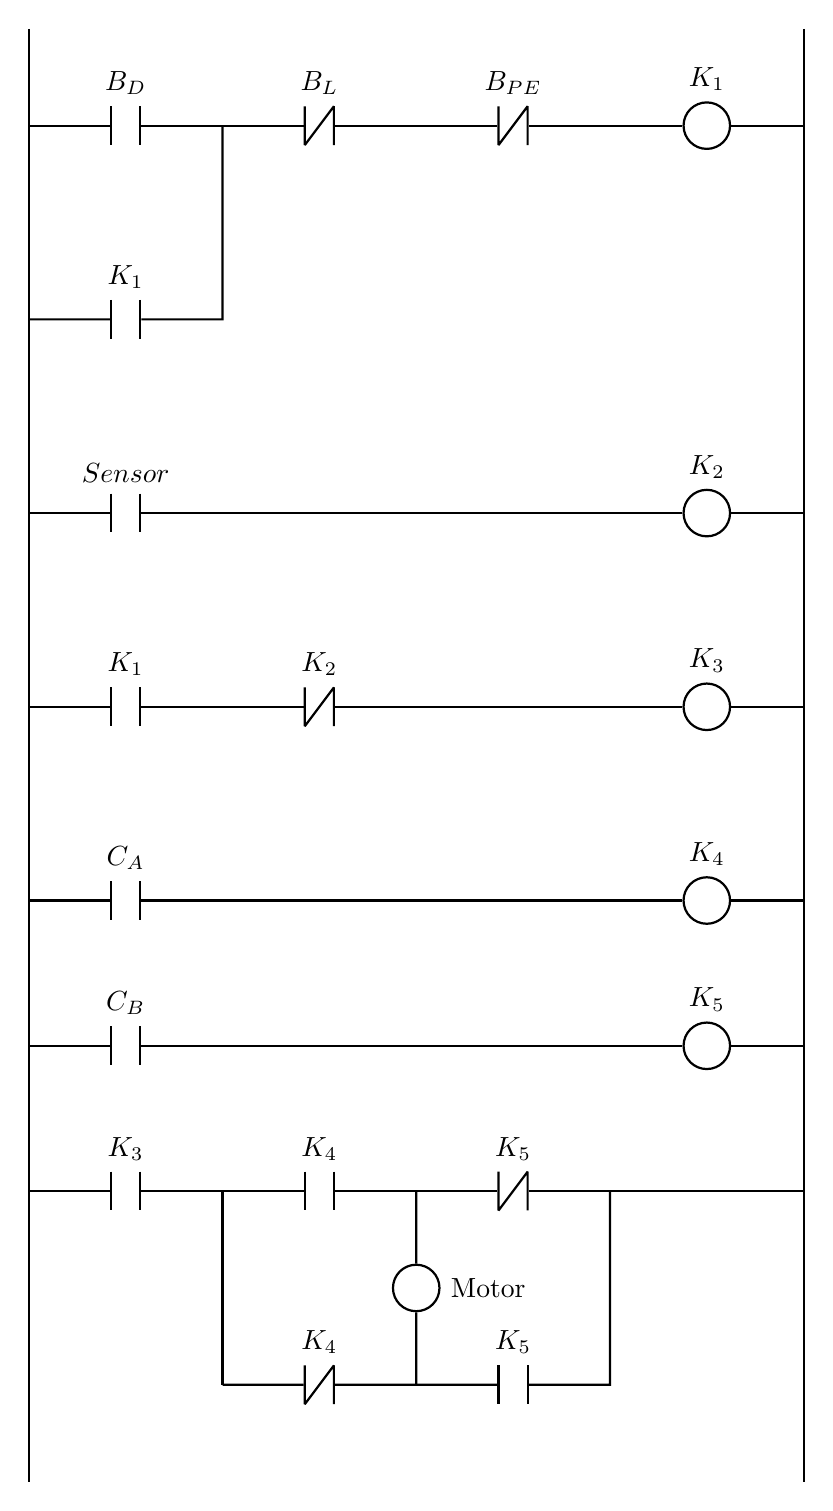
\begin{tikzpicture}[circuit plc ladder,thick]
    \draw(0,0)  to [contact NO={info={$B_D$}}] ++(2,0)
                to [contact NC={info={$B_L$}}] ++(2,0)
                to [contact NC={info={$B_{PE}$}}] ++(2,0)
                to [coil={info={$K_1$}}] ++(2,0);
    \draw(0,-2) to [contact NO={info={$K_1$}}] ++(2,0)
               -- (2,0);

    \draw(0,-4) to [contact NO={info={$Sensor$}}] ++(2,0)
                -- ++(4,0)
                to [coil={info={$K_2$}}] ++(2,0);
                
    \draw(0,-6) to [contact NO={info={$K_1$}}] ++(2,0)
                to [contact NC={info={$K_2$}}] ++(2,0)
                -- ++(2,0)
                to [coil={info={$K_3$}}] ++(2,0);
                
    \draw(0,-8) to [contact NO={info={$C_A$}}] ++(2,0)
                -- ++(4,0)
                to [coil={info={$K_4$}}] ++(2,0);
    \draw(0,-9.5) to [contact NO={info={$C_B$}}] ++(2,0)
                -- ++(4,0)
                to [coil={info={$K_5$}}] ++(2,0);
                
    \draw(0,-11) to [contact NO={info={$K_3$}}] ++(2,0)
                 to [contact NO={info={$K_4$}}] ++(2,0)
                 to [contact NC={info={$K_5$}}] ++(2,0)
                 -- ++(2,0);
    \draw(4,-11) to [coil={info={Motor}}] ++(0,-2);
    \draw(2,-13) -- ++(0,2);
    \draw(2,-13) to [contact NC={info={$K_4$}}] ++(2,0)
                 to [contact NO={info={$K_5$}}] ++(2,0)
                 -- ++(0,2);
% power rails
    \draw(0,1) -- ++(0,-15);
    \draw(8,1) -- ++(0,-15);
\end{tikzpicture}
    \caption{Diagrama Ladder sistema}
    \label{fig:my_label}
\end{figure}

\section{Conclusão}

Explorar diferentes representação usando os modelos por automatos, rede de petri e ladder permitiu um maior aprendizado sobre as particularidades de cada formato. Foi percebido que em muitos casos é possível o dialogo entre as representação, uma vez foi utilizado lógica boleana com apoio para os 3 projetos, porém a transposição entre os diferentes modelos não foi imediata.

A codificação em Linguagem C acabou ficando um pouco confusa. Embora tenha facilitado os testes de diferentes cenários de forma rápida adaptar a máquina de estados ao simulador acabou acarretando em um custo a mais na implementação.

% ------------------------------------------------------------------------------
\newpage
% Referências
\addcontentsline{toc}{section}{Referências} % Adiciona linha no índice
\bibliographystyle{abbrv} % Define Estilo e gera bibliografia
\bibliography{references} % Adiciona Arquivo com Referências

% Acrescentadas no arquivo references.bib
% para usa-las no texto basta usar \citep{}
% para citar sem usar no texto basta usar \nocite{}
%\nocite{sympy}
%\nocite{pythontex}
%\nocite{matlabcontrol}
%\nocite{matlabsymbolic}
%\nocite{ogata2010modern}
%\nocite{nise2012}

% http://ctan.math.illinois.edu/graphics/pgf/contrib/tikz-ladder/doc/tikz-ladder-doc.pdf

% ------------------------------------------------------------------------------
\newpage
\section*{Anexos}
\addcontentsline{toc}{section}{Anexos} % Adiciona linha no indice
%\subsection*{Python}

%Para os cálculos e demonstrações foi utilizado o pacote \textit{Python}\TeX\ \cite{pythontex} para o \LaTeX\ em conjunto da bibliteca \textit{sympy}\cite{sympy}. Segue o script completo em python:

%\inputminted[xleftmargin=15pt,linenos,frame=single,framesep=5pt,breaklines=true]{python}{../python/exsim6.py}

\subsection*{C}

A partir do código fornecido pelo professor foram feitas algumas modificações para permitir a implementação da máquina de estados, conforme descrito em cada parte a seguir:

\subsubsection*{Definição Estados e Eventos}
\inputminted[xleftmargin=15pt,linenos,frame=single,framesep=5pt,breaklines=true]{c}{../c/state_machine/inc/state_machine.h}

\newpage
\subsubsection*{Definição Comportamento Interno}
Foram acrescentados funções internas representando ações em um sistema real para facilitar os testes.
\inputminted[xleftmargin=15pt,linenos,frame=single,framesep=5pt,breaklines=true]{c}{../c/state_machine/src/state_machine.c}

\newpage
\subsubsection*{Definição Testes}
\inputminted[xleftmargin=15pt,linenos,frame=single,framesep=5pt,breaklines=true]{c}{../c/state_machine/src/test_1.c}

\newpage
\subsection*{Matlab}

Foi utilizado o \textit{Matlab} em conjunto da toolbox\textit{Symbolic Math}\cite{matlabsymbolic}. Para facilitar o estudo de forma interativa, o código foi dividido em múltiplos arquivos contendo funções auxiliares e um arquivo de script contendo todo a lógica usada para gerar as figuras e diagramas

\subsubsection*{Script Principal}

\inputminted[xleftmargin=15pt,linenos,frame=single,framesep=5pt,breaklines=true]{matlab}{../matlab/petrinetproject.m}

\subsubsection*{Funções Auxiliares}

Inicialmente foi definido uma função para verificar se uma transição é permitida para um determinado estado:

\inputminted[xleftmargin=15pt,linenos,frame=single,framesep=5pt,breaklines=true]{matlab}{../matlab/petristate.m}

Para avaliar as transições da Rede de Petri foi definido uma função auxiliar para gerar as árvores de transição de estados:

\inputminted[xleftmargin=15pt,linenos,frame=single,framesep=5pt,breaklines=true]{matlab}{../matlab/dotpetree.m}

% ------------------------------------------------------------------------------
\end{document}
